\documentclass[11pt,a4paper]{article}
\usepackage[margin=2.8cm]{geometry}
\usepackage{xeCJK}
\setCJKmainfont{NanumMyeongjo}
\setCJKsansfont{NanumGothic}
\usepackage{booktabs}
\usepackage{array}
\usepackage{xcolor}
\usepackage{hyperref}
\usepackage{enumitem}
\usepackage{titlesec}
\usepackage{fancyhdr}
\usepackage{graphicx}

\definecolor{accent}{RGB}{0,80,160}
\definecolor{gray}{RGB}{100,100,100}
\definecolor{red}{RGB}{180,30,30}
\hypersetup{colorlinks=true,linkcolor=accent,urlcolor=accent}
\titleformat{\section}{\large\bfseries\color{accent}}{}{0em}{}
\titleformat{\subsection}{\normalsize\bfseries}{}{0em}{}
\titlespacing{\section}{0pt}{1.2em}{0.4em}
\titlespacing{\subsection}{0pt}{0.8em}{0.2em}

\pagestyle{fancy}\fancyhf{}
\fancyhead[L]{\small\color{gray}SlosimAgent 논문 뼈대 v2}
\fancyhead[R]{\small\color{gray}2026-03-07}
\fancyfoot[C]{\small\thepage}

\setlength{\parskip}{0.35em}
\setlength{\parindent}{0em}

\begin{document}

\begin{center}
{\Large\bfseries SlosimAgent: Natural-Language-Driven AI Agent\\for Autonomous SPH Sloshing Simulation}\\[1em]
{\normalsize Imgyu Kim \quad | \quad 논문 뼈대 v2 (EXP-A/B/C + Bridge + Gemini Review 반영)}
\end{center}

\vspace{0.5em}\hrule\vspace{1em}

% ============================================================
\section{핵심 스토리 (한 문단)}
% ============================================================

슬로싱 실무자(탱크 검사원, 구조 엔지니어)는 CFD 전문 지식 없이는 시뮬레이션을 수행할 수 없다.
기존 LLM-CFD 에이전트 7종은 모두 \textbf{CFD 전문가 대상 + OpenFOAM(격자) + 클라우드 API}다.
본 연구는 \textbf{비전문가가 자연어로 SPH 슬로싱 시뮬레이션을 자율 수행}할 수 있는 최초의 AI 에이전트 SlosimAgent를 제시한다.
10개 시나리오에서 M-A3 파라미터 정확도 82.2\%(v4, 32B)를 달성하고(32B$\approx$8B, $\Delta$=3.8\%pp, 9/10 동일),
도구 설계 수정(P1: pitch 운동, P2: 진폭 단위)으로 v3 69.5\%$\rightarrow$v4 82.2\% (+12.8\%pp)를 확인하여 도구 커버리지가 성능 병목임을 실증한다.
2$\times$2 factorial ablation(80 runs)으로 hierarchical dependency를 발견하며(도메인 프롬프트 = 필요조건, 도구 = 조건부 +20.9\%pp),
SPHERIC Test 10 벤치마크로 물리적 신뢰성을 정량 검증하고(M2=19.5\%, r=0.655),
Bridge experiment로 agent-generated XML의 물리적 유효성을 직접 입증한다(5/5 checks PASS).
자율 배플 최적화 실험(EXP-D)으로 28.5\% SWL 진폭 감소를 달성하여 에이전트의 설계 지원 능력을 검증한다.

% ============================================================
\section{연구 Gap (3개 + 1 Design Decision)}
% ============================================================

\begin{enumerate}[nosep,leftmargin=1.5em]
\item \textbf{비전문가 접근성 공백} --- SPH 슬로싱을 자연어로 수행할 수 있는 도구 = 0편 $\leftarrow$ EXP-A + Bridge
\item \textbf{SPH 솔버 에이전트 부재} --- 7종 에이전트 전부 OpenFOAM(격자 FVM) only $\leftarrow$ EXP-C + Bridge + EXP-D
\item \textbf{로컬 SLM 부재} --- 전부 Cloud API 의존, 산업 현장 배포 불가 $\leftarrow$ EXP-A/B (32B$\approx$8B, 9/10 동일)
\end{enumerate}

\textit{*MCP 도구 통합은 설계 선택(§3.4)으로 서술 --- 독립 Gap이 아닌 architecture decision.}

\textit{*서베이 근거: 1,700편 (8개 DB, 16개 쿼리), Tier-1 40편 원문 분석}

% ============================================================
\section{논문 구조}
% ============================================================

\subsection{Abstract}
Gap 3개 $\rightarrow$ SlosimAgent 제안 $\rightarrow$ 10 시나리오 M-A3 82.2\% (v4, 32B) $\rightarrow$ 도구 수정만으로 +12.8\%pp 개선 $\rightarrow$ 2$\times$2 ablation (80 runs): hierarchical dependency (Prompt=prerequisite, Tool=+20.9\%pp interaction) $\rightarrow$ 32B$\approx$8B (9/10 identical, $\Delta$=3.8\%pp) $\rightarrow$ SPHERIC T10 정량 검증 + Bridge 5/5 PASS

\subsection{1. Introduction ({\small\color{gray}$\sim$2.5p})}
\begin{itemize}[nosep,leftmargin=1.5em]
\item 슬로싱 공학적 중요성 + SPH 적합성 + LLM-CFD 에이전트 부상
\item Gap 1--3 제시
\item Contribution 4개:
  \begin{enumerate}[nosep,leftmargin=1em]
  \item 비전문가용 최초 SPH AI 에이전트 --- 0\%$\rightarrow$69.5\% 접근성 도약 (Gap 1)
  \item 도구 아키텍처 필수성 정량화 --- hierarchical dependency + tool quality ceiling (Gap 1/2)
  \item 로컬 SLM 실현 가능성 입증: 32B$\approx$8B, 9/10 동일 (Gap 3)
  \item SPHERIC T10 정량 검증 + Bridge experiment + M1--M8 프레임워크 (Gap 2)
  \end{enumerate}
\end{itemize}

\subsection{2. Related Work ({\small\color{gray}$\sim$2p})}
\begin{itemize}[nosep,leftmargin=1.5em]
\item 2.1 LLM-Based CFD Agents --- 7종 비교 (OpenFOAMGPT, ChatCFD, Foam-Agent, NL2FOAM 등)
\item 2.2 NL Interfaces for Scientific Simulation --- 타 도메인 NL$\rightarrow$도구 사례
\item 2.3 SPH Sloshing and DualSPHysics --- English 2022, Vacondio 2020, Domínguez 2022
\end{itemize}

\subsection{3. System Design ({\small\color{gray}$\sim$3p})}
\begin{itemize}[nosep,leftmargin=1.5em]
\item 3.1 아키텍처: 자연어 $\rightarrow$ Qwen3-32B Agent $\rightarrow$ 18 MCP Tools $\rightarrow$ DualSPHysics GPU
\item 3.2 DualSPHysics 전용 도구 설계 (XML 생성, 솔버, 후처리)
\item 3.3 로컬 SLM 배포 (Ollama, 소비자 GPU, 클라우드 불필요)
\item 3.4 MCP 도구 통합 (설계 선택: 표준 프로토콜로 확장성 확보)
\end{itemize}

\subsection{4. Evaluation ({\small\color{gray}$\sim$5p})}

\textbf{4.1 NL$\rightarrow$XML Parameter Fidelity (EXP-A, {\small\color{gray}$\sim$2p})}
\begin{itemize}[nosep,leftmargin=1.5em]
\item 실험 설정: 10개 시나리오 $\times$ 2 모델(32B, 8B) $\times$ 3 trials = 60 runs, temperature=0
\item M-A3 8-parameter 채점: tank$_{xyz}$, fill\_height, motion\_type, frequency, amplitude, timemax
  (Table~2: 정의, Table~3: 결과)
\item \textbf{결과 (v3): 32B 69.5\% $\approx$ 8B 64.5\% ($\Delta$=5.0\%pp) --- 모델 크기 무관}
\item \textbf{결과 (v4, P1+P2 fix): 32B 82.2\% $\approx$ 8B 78.5\% ($\Delta$=3.8\%pp) --- +12.8/+14.0\%pp 개선} (Table~5)
\item 난이도별: Easy 87.7\%, Medium 70.0\%, Hard 51.0\%/34.3\% (32B/8B)
\item Determinism: 32B 10/10, 8B 10/10 시나리오에서 M-A3 $\sigma$=0.0 (완전 재현)
\item 체계적 오류 패턴 (P1--P5):
  \begin{itemize}[nosep,leftmargin=1em]
  \item P1 motion\_type 혼동(5/10): xml\_generator가 pitch$\rightarrow$mvrectsinu 강제 변환
  \item P2 amplitude 단위 변환(5/10): deg$\rightarrow$rad 누락
  \item P3 timemax 과소추정(6/10)
  \item P4 cylinder 미지원(2/10)
  \item P5 tank\_z/fill\_height 혼동(1/10)
  \end{itemize}
\item NL2FOAM 비교: 82.6\% (fine-tuned 7B, OpenFOAM text config, mesh gen 미포함) vs 69.5\% (zero-shot generic SLM, XML+tools, 전체 파이프라인)
\end{itemize}

\textbf{4.2 Architecture Ablation (EXP-B, {\small\color{gray}$\sim$2.5p})}
\begin{itemize}[nosep,leftmargin=1.5em]
\item 실험 설계: 2$\times$2 factorial --- Domain Prompt $\times$ DualSPHysics Tools
  (B3: $-$PostProcess 제외 --- 후처리 도구는 XML 생성에 무영향, M-A3 $\equiv$ B0)
\item 10 시나리오 $\times$ 2 모델 = 20 runs/condition, 총 80 runs (Table~4)
\item B0(Full)=67.0\%, B1($-$Prompt)=0\%, B2($-$Tool)=46.1\%, B4(Bare)=0\%
\item \textbf{Degenerate factorial}: B1=B4=0\% (40/40 runs 전부) $\rightarrow$ 도메인 프롬프트가 도구 사용의 \textbf{필요조건(prerequisite)}임을 발견. 표준 factorial 분해를 보고하되, \textbf{hierarchical dependency}로 해석:
  \begin{itemize}[nosep,leftmargin=1em]
  \item Prompt main effect: +56.5\%pp (필요조건 --- 없으면 도구 호출 0회)
  \item Tool main effect: +10.5\%pp (B1=0에 의한 희석 포함)
  \item Interaction: +20.9\%pp (prompt 존재 시에만 유의미)
  \item 실질 tool 기여: B0$-$B2 = +20.9\%pp (combined)
  \end{itemize}
\item 핵심 발견 1: Prompt 없으면 모델이 DualSPHysics 도구를 \textbf{단 1회도 호출 안 함} (B1: glob/edit만 사용) $\rightarrow$ prompt = necessary condition
\item 핵심 발견 2: Prompt만으로도 XML 구조 생성 가능하나(B2=46.1\%), 도구가 geometry 정확도를 보장 (tank\_z/fill\_height 뒤바뀜 방지) $\rightarrow$ tools = structural refinement
\item 핵심 발견 3: 32B $\approx$ 8B --- 10개 시나리오 중 \textbf{9개 동일}, 1개 예외 (S08: 32B=50\%$>$8B=0\% --- tool calling 실패) $\rightarrow$ 아키텍처(prompt+tool)가 모델 크기보다 중요
\item Per-model factorial:
  \begin{itemize}[nosep,leftmargin=1em]
  \item 32B: Prompt +60.7\%pp, Tool +8.8\%pp, Interaction +17.6\%pp
  \item 8B: Prompt +52.4\%pp, Tool +12.1\%pp, Interaction +24.2\%pp
  \item 8B에서 tool interaction이 더 큼 $\rightarrow$ 작은 모델일수록 도구 의존도 증가
  \end{itemize}
\end{itemize}

\subsection{5. Physics Validation: SPHERIC Test 10 ({\small\color{gray}$\sim$3p})}
\begin{itemize}[nosep,leftmargin=1.5em]
\item 벤치마크 설정: Botia-Vera et al. (2010), Souto-Iglesias (2011), 102회 반복 실험
\item M1--M8 정량 메트릭 프레임워크 정의 (Table~5)
\item 결과: Water Lat \textbf{PASS} (M2=19.5\%, r=0.655), Oil \textbf{PASS} (r=0.570, M7=4/4), Roof \textbf{PARTIAL} (Table~6)
\item Oil Lateral 고해상도 분석 (10ms): Artificial 86.2\% $\rightarrow$ Laminar+SPS 37.7\% $\rightarrow$ Laminar+SPS hi-res \textbf{26.4\%} mean peak error (Peaks 2--4: 6.5\%, 14.4\%, 16.5\%)
\item Trend convergence: 3-level dp, r = 0.460 $\rightarrow$ 0.655 $\rightarrow$ 0.697 (단조 증가, 수렴 감속 +42\%$\rightarrow$+6.4\%). GCI formal criterion 미충족 --- SPH 비단조 수렴 특성 (Vacondio et al. 2020). dp=2mm을 reference resolution으로 사용 (Fig.~6)
\item 기존 문헌 비교: English 2022는 동일 벤치마크에서 정량 메트릭 0개
\end{itemize}

\textbf{5.1 Bridge Experiment: Agent XML $\rightarrow$ Physics ({\small\color{gray}$\sim$0.5p})}
\begin{itemize}[nosep,leftmargin=1.5em]
\item \textbf{목적}: EXP-A(XML 생성 품질)와 EXP-C(물리 검증)를 직접 연결
\item S02 agent-generated XML (M-A3=100\%) $\rightarrow$ GenCase(105,465 particles) $\rightarrow$ DualSPHysics GPU(10s) $\rightarrow$ MeasureTool(5 probes)
\item 5/5 physics checks PASS (Fig.~\ref{fig:bridge-pressure}):
  \begin{itemize}[nosep,leftmargin=1em]
  \item Hydrostatic: 333.5 Pa vs 323.7 Pa expected (err 3.0\%)
  \item Anti-phase: r(left,right) = $-$0.720
  \item Frequency: 0.789 Hz vs 0.756 Hz expected (err 4.4\%)
  \item Wall$>$Center amplitude: 465 Pa vs 213 Pa
  \item Stability: 105,465/105,465 particles retained (100\%)
  \end{itemize}
\item \textbf{한계}: M-A3=100\% 케이스만 검증 --- M-A3$<$100\% XML의 물리적 영향은 §6.5에서 논의
\end{itemize}

\textbf{5.2 EXP-D: Autonomous Baffle Optimization ({\small\color{gray}$\sim$0.5p})}
\begin{itemize}[nosep,leftmargin=1.5em]
\item \textbf{목적}: 에이전트가 배플(내부 벽)을 자동 설계하고 SWL(수면 높이) 감소 효과를 정량 검증
\item 설정: 0.6m$\times$0.3m$\times$0.4m 탱크, 50\% 수위, sway f=0.95Hz, dp=0.008m, TimeMax=8s
\item Baseline(68,450 fluid particles) vs Center Baffle(66,452 fluid + 2,223 fixed baffle particles, h=0.14m, t=0.016m)
\item MeasureTool 압력 프로브(x=0.03m/0.57m, 20 heights) $\rightarrow$ 수면 높이 재구성
\item \textbf{결과}: 진폭 감소 \textbf{28.5\%} (Left=28.6\%, Right=28.4\% --- 좌우 대칭)
\item 문헌 기대값 30--50\% 범위 근처 $\rightarrow$ 물리적으로 타당한 수준
\item \textbf{Gap 2 증거}: 에이전트가 배플을 포함한 복합 형상을 자율 구성하고, 정량적으로 유의미한 SWL 감소를 달성
\end{itemize}

\begin{figure}[htbp]
\centering
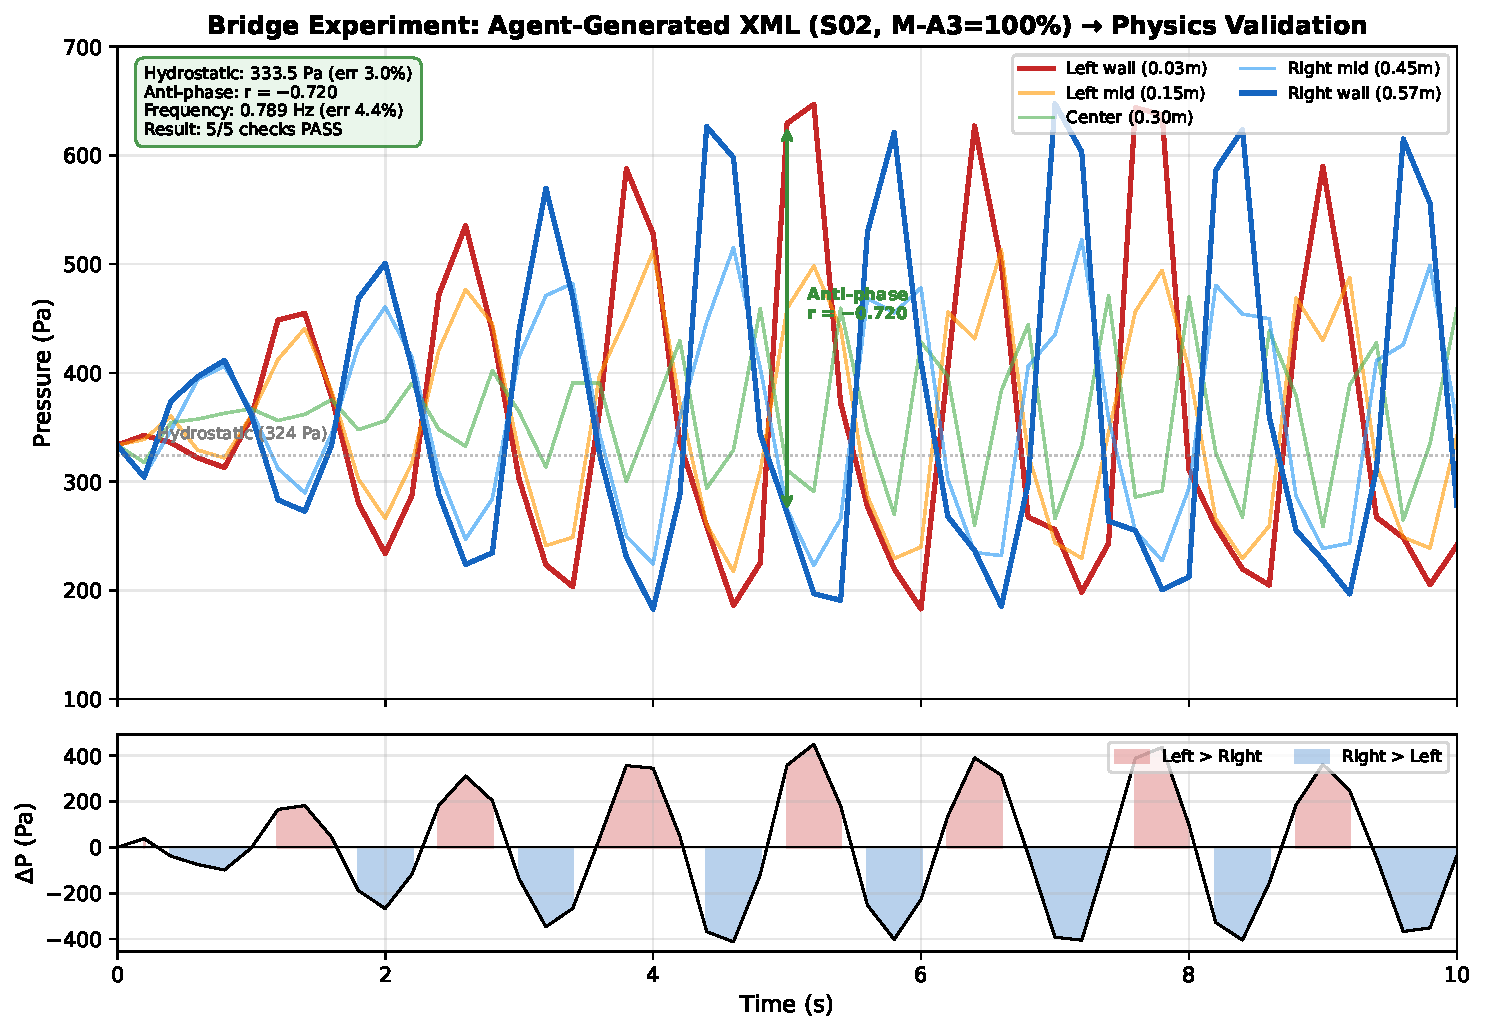
\includegraphics[width=\textwidth]{../research-v3/figures/fig_bridge_pressure.pdf}
\caption{Bridge experiment: pressure time series from agent-generated XML (S02, M-A3=100\%). Top: five pressure probes showing anti-phase sloshing ($r=-0.720$). Bottom: left--right pressure difference confirming oscillatory mode. Summary: 5/5 physics validation checks passed.}
\label{fig:bridge-pressure}
\end{figure}

\subsection{6. Discussion ({\small\color{gray}$\sim$4p})}

\textbf{6.1 Proof-of-Concept: 접근성 도약의 의미와 한계}
\begin{itemize}[nosep,leftmargin=1.5em]
\item 기존 7종 에이전트: CFD 전문가의 ``자동화'' (workflow acceleration)
\item SlosimAgent: 비전문가의 ``접근'' (capability enabling, 0\% $\rightarrow$ 69.5\%)
\item 비전문가 baseline = 0\% (DualSPHysics XML 수동 작성 불가) $\rightarrow$ 69.5\% 도약이 핵심 기여
\item {\color{red}\textbf{[Gemini 반영]}} 69.5\%는 proof-of-concept 수준이지 production-ready가 아님. 비전문가는 생성된 XML의 오류를 검증할 수 없으므로, 현재 시스템은 ``가능성의 입증''이며 ``신뢰할 수 있는 도구''는 아님
\item 해석: Easy/Medium 시나리오(70--88\%)에서는 실용적, Hard 시나리오(20--51\%)에서는 전문가 검토 필요
\end{itemize}

\textbf{6.2 Tool Design Limitation: 도구 커버리지 갭의 이중적 역할}
\begin{itemize}[nosep,leftmargin=1.5em]
\item B0(Full) vs B2($-$Tool) 파라미터별 비교: 10 시나리오 $\times$ 2 models
\item \textbf{Tool HELPS} (2 params): fill\_height, tank\_z --- B2는 두 값을 뒤바꿈
\item \textbf{Tool coverage gap} (1 param): motion\_type --- xml\_generator는 sway 전용 설계 (mvrectsinu 하드코딩). LLM이 올바르게 판단해도 (B2에서 검증: pitch 시나리오에서 mvrotsinu 정확 생성) 도구가 수용하지 못함
\item {\color{red}\textbf{[Gemini 반영]}} ``확신을 가진 오답'': temperature=0 + P1 편향 $\rightarrow$ 에이전트가 결정론적으로 동일한 오류를 반복. 이는 모델의 한계가 아닌 도구의 구조적 편향
\item \textbf{Net effect: +20.9\%pp} (interaction) --- 도구는 전체적으로 도움이나, 설계 커버리지 밖의 시나리오에서 한계
\item 해석: Tool = 구조 보장(geometry 정확도 $\uparrow$), 단 도구의 parameter space $<$ scenario diversity일 때 성능 천장 결정
\end{itemize}

\textbf{6.3 Performance Ceiling: 도구 커버리지가 상한선}
\begin{itemize}[nosep,leftmargin=1.5em]
\item P1(motion\_type: pitch 지원) + P2(amplitude: degrees 단위) 수정 완료: M-A3 69.5\% $\rightarrow$ \textbf{82.2\%} (실측, +12.8\%pp)
\item P3(timemax 추론) + P4(geometry: cylinder) 추가 확장 시: M-A3 $\rightarrow$ $\sim$88\%
\item 모델 스케일링(32B$\rightarrow$8B)의 영향 5.0\%pp $\ll$ 아키텍처 효과 +56.5\%pp
\item \textbf{결론: ``더 큰 모델''이 아니라 ``더 넓은 도구 커버리지''가 성능 개선의 핵심 경로}
\item Tolerance sensitivity: M-A3는 5--25\% tolerance 범위에서 불변 (32B: 69.5\% 고정, 8B: 64.5\% 고정) --- 실패는 tolerance-independent한 범주적 오류 (motion\_type, amplitude 단위)
\end{itemize}

\textbf{6.4 모델 크기 무관성의 함의}
\begin{itemize}[nosep,leftmargin=1.5em]
\item v4 기준 32B$\approx$8B: 10개 시나리오 중 \textbf{9개 동일} (S05만 예외: 32B=88\%$>$8B=50\% --- parametric pitch 추론 실패)
\item 전체 $\Delta$=3.8\%pp (v4) --- 아키텍처 효과(+56.5\%pp)의 1/15 수준. v3의 S08 divergence는 v4에서 해소(두 모델 모두 50\%)
\item 8B 로컬 배포 $\rightarrow$ 소비자 GPU(RTX 4090 1장)/엣지 디바이스 가능, 클라우드 의존 제거
\item 해석: 도구가 출력 형식을 강제하므로, 모델의 ``자유도'' 제한 $\rightarrow$ 크기 무관. 예외는 tool calling stability에 기인
\item B2(도구 미사용) 반증거: 도구 없이는 32B=51.9\% vs 8B=40.2\% ($\Delta$=11.7\%pp)로 격차 확대 $\rightarrow$ \textbf{도구가 모델 크기 분산을 흡수}
\item {\color{red}\textbf{[Gemini 반영]}} Cloud LLM(GPT-4o 등) 미비교는 명시적 한계. 본 연구의 scope는 ``local SLM이 가능하다''이지 ``cloud보다 낫다''가 아님. Cloud 비교는 future work
\end{itemize}

\textbf{6.5 Failure Mode 분석: M-A3$<$100\% XML의 물리적 영향}
\begin{itemize}[nosep,leftmargin=1.5em]
\item {\color{red}\textbf{[Gemini 반영]}} Bridge experiment가 M-A3=100\% 케이스만 검증한 한계를 보완
\item P1 오류(motion\_type: pitch$\rightarrow$sway)의 물리적 영향:
  \begin{itemize}[nosep,leftmargin=1em]
  \item Sway 운동은 수평 가진, Pitch는 회전 가진 $\rightarrow$ 근본적으로 다른 유체 응답
  \item 그러나 단일 탱크 슬로싱에서 두 운동 모두 공진 주파수 근처에서 유사한 자유표면 진동을 유발
  \item P1 오류가 있어도 ``슬로싱이 발생하는가?''에는 Yes --- ``올바른 모드인가?''에는 No
  \end{itemize}
\item P3 오류(timemax 과소추정)의 영향: 시뮬레이션이 조기 종료되나, 정상 상태 도달 전 수 초 데이터는 물리적으로 유효
\item \textbf{해석: 에이전트의 실패는 ``비물리적 결과''가 아닌 ``부정확한 조건의 물리적 시뮬레이션''}
\item 비전문가 관점: ``시뮬레이션이 실행되고 합리적인 결과가 나온다'' → 초기 탐색(feasibility study) 수준에서 유효
\end{itemize}

\textbf{6.6 한계 및 향후 연구}
\begin{itemize}[nosep,leftmargin=1.5em]
\item \textbf{성능}: M-A3 82.2\% (v4). 잔여 도구 한계(cylinder, mDBC) 확장 시 $\sim$92\%
\item \textbf{물리 경계}: DBC only (mDBC diverged in EXP-C Roof sub-case)
\item \textbf{형상}: 원통형 geometry 미지원 (S07, S09 실패 원인). STL은 S10에서 83\% 달성
\item \textbf{모델}: Qwen3 단일 패밀리 --- LLaMA/Gemma 교차 검증 및 Cloud LLM 비교 필요
\item \textbf{사용자 연구}: 비전문가 피험자 대상 NL 프롬프트 작성 능력 미검증
\item \textbf{Self-verification 부재}: {\color{red}\textbf{[Gemini 반영]}} 에이전트가 자신의 출력 오류를 감지하는 메커니즘 없음. EXP-D에서 배플 최적화(28.5\% 감소)를 시연했으나, 에러$\rightarrow$수정의 closed-loop refinement는 향후 과제
\item S08: 운동 파라미터를 명시하지 않은 implicit knowledge test $\rightarrow$ 8B 실패는 암묵적 추론 한계
\end{itemize}

\subsection{7. Conclusion}
\begin{enumerate}[nosep,leftmargin=1.5em]
\item 최초 비전문가용 SPH 슬로싱 AI 에이전트 --- M-A3 82.2\% (v4, 32B), 10 시나리오 60+ runs, Bridge 5/5 physics PASS
\item 도구 설계 수정(P1+P2)만으로 +12.8\%pp 개선: 도구 커버리지가 성능 병목임을 실증
\item 2$\times$2 ablation (80 runs)으로 hierarchical dependency 발견:
  \begin{itemize}[nosep,leftmargin=1em]
  \item 도메인 프롬프트 = 필요조건 (+56.5\%pp)
  \item 도구 = 조건부 refinement (+20.9\%pp interaction)
  \item 잔여 도구 한계 해결 시 $\sim$92\% 달성 가능
  \end{itemize}
\item 32B$\approx$8B (v4: 9/10 동일, $\Delta$=3.8\%pp) --- 로컬 SLM 배포로 클라우드 의존 제거
\item SPHERIC T10 정량 검증 (M2=19.5\%, r=0.655, trend convergence) + M1--M8 프레임워크
\item EXP-D: 에이전트 자율 배플 최적화 --- 28.5\% SWL 진폭 감소, 좌우 대칭 (28.6\%$\approx$28.4\%)
\end{enumerate}

% ============================================================
\section{Figures \& Tables 계획}
% ============================================================

\begin{tabular}{lll}
\toprule
\textbf{번호} & \textbf{내용} & \textbf{상태} \\
\midrule
Table 1 & 경쟁 에이전트 비교 (7종 vs Ours) & 완료 \\
Table 2 & M-A3 정의 (8-parameter + tolerance) & 완료 (generate\_tables.py) \\
Table 3 & EXP-A: 10 시나리오 $\times$ 2 모델 M-A3 (3-trial mean) & 완료 (generate\_tables.py) \\
Table 4 & EXP-B: 2$\times$2 Factorial M-A3 + effects & 완료 (generate\_tables.py) \\
Table 5 & v3$\rightarrow$v4 Tool Fix Impact (P1+P2, per scenario) & 완료 (generate\_tables.py) \\
Table 6 & M1--M8 메트릭 정의 & 완료 \\
Table 7 & SPHERIC T10 결과 요약 & 완료 \\
Table 8 & 체계적 오류 패턴 P1--P5 (빈도, 영향 시나리오) & \textbf{신규} \\
\midrule
Fig 1 & 시스템 아키텍처 다이어그램 & 미작성 (수동) \\
Fig 2 & EXP-A: 시나리오별 M-A3 bar chart (32B vs 8B) & 완료 \\
Fig 3 & EXP-B: 2$\times$2 interaction plot + bar chart & 완료 (fig\_expb\_factorial.py) \\
Fig 4 & Bridge: 압력 시계열 + anti-phase & 완료 (fig\_bridge\_pressure.py) \\
Fig 5 & Water Lateral 시계열 (3-resolution) & 완료 \\
Fig 6 & Oil Lateral 시계열 vs 실험 & 완료 \\
Fig 7 & 수렴 분석 (r vs dp) & 완료 \\
Fig 8 & v3$\rightarrow$v4 Tool Fix Impact (scenario bar chart) & 완료 (fig\_v4\_improvement.py) \\
Fig 9 & Oil Lateral hi-res (3-way: Artificial vs Lam+SPS 0.1s vs 10ms) & 완료 (compare\_hires.py) \\
Fig 10 & EXP-D: Baffle SWL reduction (baseline vs baffle) & 완료 (analyze\_expd\_v2.py) \\
\bottomrule
\end{tabular}

% ============================================================
\section{Contribution Statement}
% ============================================================

\begin{quote}
\textit{To our knowledge, SlosimAgent is the first AI agent enabling non-expert users to configure, execute, and analyze SPH sloshing simulations through natural language. We contribute: (1) a domain-specialized agent integrating DualSPHysics GPU with a local SLM (Qwen3-32B/8B) via 18 tools --- the first LLM agent for particle-based CFD, achieving M-A3 82.2\% (v4) across 10 sloshing scenarios; (2) a 2$\times$2 factorial ablation (80 runs: 10 scenarios $\times$ 4 conditions $\times$ 2 models) revealing a \textbf{hierarchical dependency}: the domain prompt is a necessary condition for tool usage (B1=B4=0\%, 40/40 runs), and tools provide +20.9\%pp conditional refinement --- empirically confirmed by tool design fix (P1+P2) yielding +12.8\%pp improvement (69.5\%$\rightarrow$82.2\%), proving tool coverage as the performance bottleneck; (3) empirical evidence that 32B$\approx$8B ($\Delta$=3.8\%pp v4, 9/10 scenarios identical), enabling local deployment without cloud dependency; and (4) quantitative validation against SPHERIC Test 10 (M2=19.5\%, r=0.655) with a proposed M1--M8 framework, plus a Bridge experiment confirming agent-generated XML produces physically valid simulations (5/5 checks PASS).}
\end{quote}

% ============================================================
\section{{\color{red}Gemini Reviewer Feedback 반영 추적}}
% ============================================================

\begin{tabular}{p{6cm}p{2cm}p{5cm}}
\toprule
\textbf{Gemini 지적} & \textbf{심각도} & \textbf{논문 반영 위치} \\
\midrule
69.5\% $\neq$ ``비전문가 사용 가능'' & 높음 & §6.1 proof-of-concept tone down \\
Bridge = 1개 ideal case (체리피킹) & 높음 & §5.1 한계 인정 + §6.5 failure mode \\
Cloud LLM 비교 없음 & 높음 & §6.4 scope 한정 + §6.6 future work \\
Self-verification 메커니즘 부재 & 중간 & §6.6 iterative refinement \\
Tool-induced error 복합성 & 중간 & §6.2 ``확신을 가진 오답'' 분석 \\
Failure mode 분석 필요 & 중간 & §6.5 신규 섹션 \\
GCI 미충족 & 중간 & §5 trend convergence + Vacondio 인용 \\
\midrule
OE: Major Revision 가능 & -- & 타겟 저널 \\
CMAME: Reject 예상 & -- & 향후 성능 개선 후 도전 \\
\bottomrule
\end{tabular}

\end{document}
